\centering
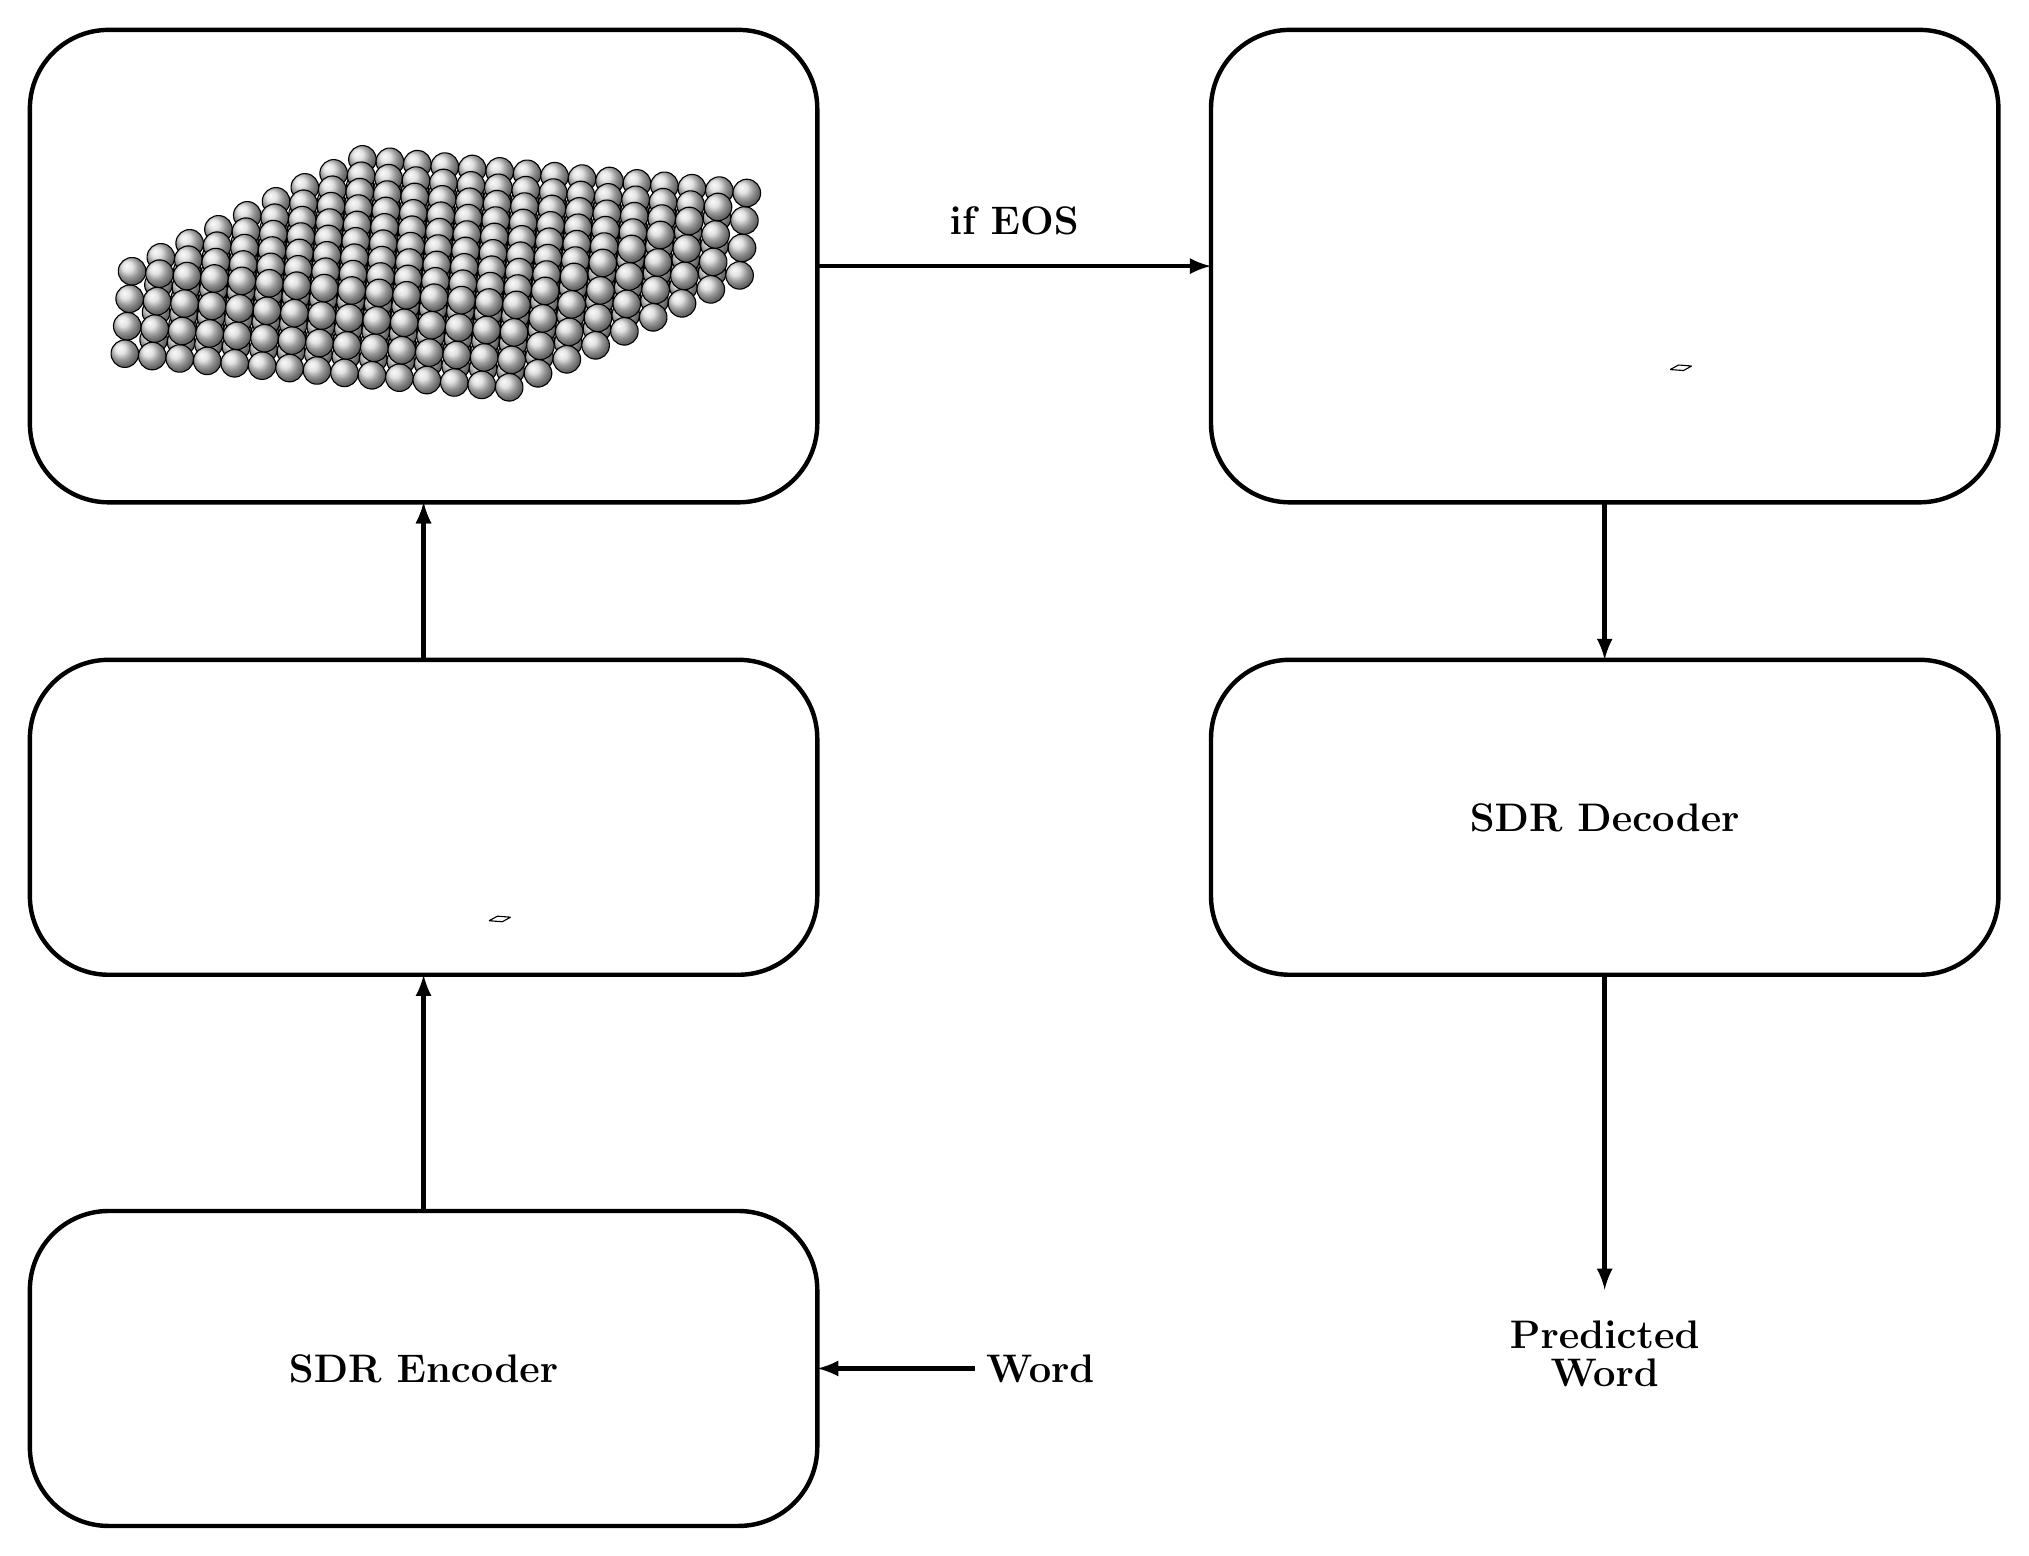
\begin{tikzpicture}



\draw[-latex,ultra thick] (6,-12) to node [right=1cm] {\Large\textbf{Word}} (4,-12);

\draw [rounded corners=1cm,ultra thick] (-6,-14) rectangle ++(10,4) node [midway] {\Large\textbf{SDR Encoder}};


\draw[-latex,ultra thick](-1,-10) to (-1,-7);



\draw [rounded corners=1cm,ultra thick] (-6,-7) rectangle ++(10,4) node [midway] {};
\begin{scope}[yshift=-180,yslant=.55,xslant=-1.6,scale=0.105]
        \ColorCells
        \draw (0, 0) grid (\GridSize, \GridSize);
        \coordinate (input);
\end{scope}

\draw[-latex,ultra thick](-1,-3) to (-1,-1);


\draw [rounded corners=1cm,ultra thick] (9,-1) rectangle ++(10,6) node [midway] {};
\begin{scope}[xshift=15cm, yshift=7cm, yshift=-180, yslant=.55, xslant=-1.6, scale=0.105] 
    \ColorCells
    \draw (0, 0) grid (\GridSize, \GridSize);
    \coordinate (output);
\end{scope}  


\draw[-latex,ultra thick](-1,-3) to (-1,-1);

\draw[-latex,ultra thick] (4,2) to node [above=.25cm] {\Large\textbf{if EOS}} (9,2);


\draw[-latex,ultra thick](14,-1) to (14,-3);

\draw [rounded corners=1cm,ultra thick] (9,-7) rectangle ++(10,4) node [midway] {\Large\textbf{SDR Decoder}};


\draw[-latex,ultra thick] (14,-7) to node [below=2.25cm] {\begin{tabular}{c} \Large\textbf{Predicted} \\ \Large\textbf{Word} \end{tabular}} (14,-11);


\draw [rounded corners=1cm,ultra thick] (-6,-1) rectangle ++(10,6) node [midway] {};

\begin{scope}[rotate around = {-5:(0,20,20)}, yshift=2.5cm,xshift=-0.5cm,scale=0.7]
   
    \foreach \x  in {0.75,1.25,1.75,2.25,2.75,3.25,3.75,4.25,4.75,5.25,5.75,6.25,6.75,7.25,7.75}%
        \shadedraw [ball color= gray!30] (\x,2,1.55*2.5) circle (0.25cm);
    \foreach \x  in {0.75,1.25,1.75,2.25,2.75,3.25,3.75,4.25,4.75,5.25,5.75,6.25,6.75,7.25,7.75}%
        \shadedraw [ball color= gray!30] (\x-.2,2,1.55*3) circle (0.25cm);
    \foreach \x  in {0.75,1.25,1.75,2.25,2.75,3.25,3.75,4.25,4.75,5.25,5.75,6.25,6.75,7.25,7.75}%
        \shadedraw [ball color= gray!30] (\x-.4,2,1.55*3.5) circle (0.25cm);
    \foreach \x  in {0.75,1.25,1.75,2.25,2.75,3.25,3.75,4.25,4.75,5.25,5.75,6.25,6.75,7.25,7.75}%
        \shadedraw [ball color= gray!30] (\x-.6,2,1.55*4) circle (0.25cm);
    \foreach \x  in {0.75,1.25,1.75,2.25,2.75,3.25,3.75,4.25,4.75,5.25,5.75,6.25,6.75,7.25,7.75}%
        \shadedraw [ball color= gray!30] (\x-.8,2,1.55*4.5) circle (0.25cm);
    \foreach \x  in {0.75,1.25,1.75,2.25,2.75,3.25,3.75,4.25,4.75,5.25,5.75,6.25,6.75,7.25,7.75}%
        \shadedraw [ball color= gray!30] (\x-1,2,1.55*5) circle (0.25cm);
    \foreach \x  in {0.75,1.25,1.75,2.25,2.75,3.25,3.75,4.25,4.75,5.25,5.75,6.25,6.75,7.25,7.75}%
        \shadedraw [ball color= gray!30] (\x-1.2,2,1.55*5.5) circle (0.25cm);
    \foreach \x  in {0.75,1.25,1.75,2.25,2.75,3.25,3.75,4.25,4.75,5.25,5.75,6.25,6.75,7.25,7.75}%
        \shadedraw [ball color= gray!30] (\x-1.4,2,1.55*6) circle (0.25cm);
    \foreach \x  in {0.75,1.25,1.75,2.25,2.75,3.25,3.75,4.25,4.75,5.25,5.75,6.25,6.75,7.25,7.75}%
        \shadedraw [ball color= gray!30] (\x-1.6,2,1.55*6.5) circle (0.25cm);


    \foreach \x  in {0.75,1.25,1.75,2.25,2.75,3.25,3.75,4.25,4.75,5.25,5.75,6.25,6.75,7.25,7.75}%
        \shadedraw [ball color= gray!30] (\x,2.5,1.55*2.5) circle (0.25cm);
    \foreach \x  in {0.75,1.25,1.75,2.25,2.75,3.25,3.75,4.25,4.75,5.25,5.75,6.25,6.75,7.25,7.75}%
        \shadedraw [ball color= gray!30] (\x-.2,2.5,1.55*3) circle (0.25cm);
    \foreach \x  in {0.75,1.25,1.75,2.25,2.75,3.25,3.75,4.25,4.75,5.25,5.75,6.25,6.75,7.25,7.75}%
        \shadedraw [ball color= gray!30] (\x-.4,2.5,1.55*3.5) circle (0.25cm);
    \foreach \x  in {0.75,1.25,1.75,2.25,2.75,3.25,3.75,4.25,4.75,5.25,5.75,6.25,6.75,7.25,7.75}%
        \shadedraw [ball color= gray!30] (\x-.6,2.5,1.55*4) circle (0.25cm);
    \foreach \x  in {0.75,1.25,1.75,2.25,2.75,3.25,3.75,4.25,4.75,5.25,5.75,6.25,6.75,7.25,7.75}%
        \shadedraw [ball color= gray!30] (\x-.8,2.5,1.55*4.5) circle (0.25cm);
    \foreach \x  in {0.75,1.25,1.75,2.25,2.75,3.25,3.75,4.25,4.75,5.25,5.75,6.25,6.75,7.25,7.75}%
        \shadedraw [ball color= gray!30] (\x-1,2.5,1.55*5) circle (0.25cm);
    \foreach \x  in {0.75,1.25,1.75,2.25,2.75,3.25,3.75,4.25,4.75,5.25,5.75,6.25,6.75,7.25,7.75}%
        \shadedraw [ball color= gray!30] (\x-1.2,2.5,1.55*5.5) circle (0.25cm);
    \foreach \x  in {0.75,1.25,1.75,2.25,2.75,3.25,3.75,4.25,4.75,5.25,5.75,6.25,6.75,7.25,7.75}%
        \shadedraw [ball color= gray!30] (\x-1.4,2.5,1.55*6) circle (0.25cm);
    \foreach \x  in {0.75,1.25,1.75,2.25,2.75,3.25,3.75,4.25,4.75,5.25,5.75,6.25,6.75,7.25,7.75}%
        \shadedraw [ball color= gray!30] (\x-1.6,2.5,1.55*6.5) circle (0.25cm);


    \foreach \x  in {0.75,1.25,1.75,2.25,2.75,3.25,3.75,4.25,4.75,5.25,5.75,6.25,6.75,7.25,7.75}%
        \shadedraw [ball color= gray!30] (\x,3,1.55*2.5) circle (0.25cm);
    \foreach \x  in {0.75,1.25,1.75,2.25,2.75,3.25,3.75,4.25,4.75,5.25,5.75,6.25,6.75,7.25,7.75}%
        \shadedraw [ball color= gray!30] (\x-.2,3,1.55*3) circle (0.25cm);
    \foreach \x  in {0.75,1.25,1.75,2.25,2.75,3.25,3.75,4.25,4.75,5.25,5.75,6.25,6.75,7.25,7.75}%
        \shadedraw [ball color= gray!30] (\x-.4,3,1.55*3.5) circle (0.25cm);
    \foreach \x  in {0.75,1.25,1.75,2.25,2.75,3.25,3.75,4.25,4.75,5.25,5.75,6.25,6.75,7.25,7.75}%
        \shadedraw [ball color= gray!30] (\x-.6,3,1.55*4) circle (0.25cm);
    \foreach \x  in {0.75,1.25,1.75,2.25,2.75,3.25,3.75,4.25,4.75,5.25,5.75,6.25,6.75,7.25,7.75}%
        \shadedraw [ball color= gray!30] (\x-.8,3,1.55*4.5) circle (0.25cm);
    \foreach \x  in {0.75,1.25,1.75,2.25,2.75,3.25,3.75,4.25,4.75,5.25,5.75,6.25,6.75,7.25,7.75}%
        \shadedraw [ball color= gray!30] (\x-1,3,1.55*5) circle (0.25cm);
     \foreach \x  in {0.75,1.25,1.75,2.25,2.75,3.25,3.75,4.25,4.75,5.25,5.75,6.25,6.75,7.25,7.75}%
        \shadedraw [ball color= gray!30] (\x-1.2,3,1.55*5.5) circle (0.25cm);
    \foreach \x  in {0.75,1.25,1.75,2.25,2.75,3.25,3.75,4.25,4.75,5.25,5.75,6.25,6.75,7.25,7.75}%
        \shadedraw [ball color= gray!30] (\x-1.4,3,1.55*6) circle (0.25cm);
    \foreach \x  in {0.75,1.25,1.75,2.25,2.75,3.25,3.75,4.25,4.75,5.25,5.75,6.25,6.75,7.25,7.75}%
        \shadedraw [ball color= gray!30] (\x-1.6,3,1.55*6.5) circle (0.25cm);
    
    
    
    \foreach \x  in {0.75,1.25,1.75,2.25,2.75,3.25,3.75,4.25,4.75,5.25,5.75,6.25,6.75,7.25,7.75}%
        \shadedraw [ball color= gray!30] (\x,3.5,1.55*2.5) circle (0.25cm);
    \foreach \x  in {0.75,1.25,1.75,2.25,2.75,3.25,3.75,4.25,4.75,5.25,5.75,6.25,6.75,7.25,7.75}%
        \shadedraw [ball color= gray!30] (\x-.2,3.5,1.55*3) circle (0.25cm);
    \foreach \x  in {0.75,1.25,1.75,2.25,2.75,3.25,3.75,4.25,4.75,5.25,5.75,6.25,6.75,7.25,7.75}%
        \shadedraw [ball color= gray!30] (\x-.4,3.5,1.55*3.5) circle (0.25cm);
    \foreach \x  in {0.75,1.25,1.75,2.25,2.75,3.25,3.75,4.25,4.75,5.25,5.75,6.25,6.75,7.25,7.75}%
        \shadedraw [ball color= gray!30] (\x-.6,3.5,1.55*4) circle (0.25cm);
    \foreach \x  in {0.75,1.25,1.75,2.25,2.75,3.25,3.75,4.25,4.75,5.25,5.75,6.25,6.75,7.25,7.75}%
        \shadedraw [ball color= gray!30] (\x-.8,3.5,1.55*4.5) circle (0.25cm);
    \foreach \x  in {0.75,1.25,1.75,2.25,2.75,3.25,3.75,4.25,4.75,5.25,5.75,6.25,6.75,7.25,7.75}%
        \shadedraw [ball color= gray!30] (\x-1,3.5,1.55*5) circle (0.25cm);
    \foreach \x  in {0.75,1.25,1.75,2.25,2.75,3.25,3.75,4.25,4.75,5.25,5.75,6.25,6.75,7.25,7.75}%
        \shadedraw [ball color= gray!30] (\x-1.2,3.5,1.55*5.5) circle (0.25cm);
    \foreach \x  in {0.75,1.25,1.75,2.25,2.75,3.25,3.75,4.25,4.75,5.25,5.75,6.25,6.75,7.25,7.75}%
        \shadedraw [ball color= gray!30] (\x-1.4,3.5,1.55*6) circle (0.25cm);
    \foreach \x  in {0.75,1.25,1.75,2.25,2.75,3.25,3.75,4.25,4.75,5.25,5.75,6.25,6.75,7.25,7.75}%
        \shadedraw [ball color= gray!30] (\x-1.6,3.5,1.55*6.5) circle (0.25cm); 
\end{scope}
\end{tikzpicture}